\chapter{基于FAST-LIO2的激光里程计定位算法研究}
\section{引言}
稳定可靠的自身定位是移动机器人在复杂动态环境中完成运输、巡检、侦察和辅助作业的前提。机器人只有在统一坐标系下持续获得准确的全局位姿，才能为后续的环境感知、障碍物检测与路径规划提供可信的空间基准。厂房、仓储空间、地下通道和大型设施内部往往结构重复、纹理单一且GNSS信号受限，单纯依靠轮式里程计或二维激光定位难以长期维持精度，容易产生累积漂移并在退化区域失效。因此，需要一种能够融合多源信息、在已知环境中提供稳定绝对定位的方法。

实时定位与地图构建（Simultaneous Localization and Mapping，SLAM）是移动机器人与自动驾驶领域的核心技术。其核心任务可归结为一种耦合估计问题：在未知环境中，移动平台利用传感器数据，同步完成对自身运动状态的描述与对环境空间结构的建模。二者相互依赖，定位精度依赖于地图的准确性，而一致地图的构建又需以精确的位姿轨迹为前提。在众多SLAM方案中，紧耦合激光惯性里程计因其高精度、低延迟和对退化环境的鲁棒性，逐渐成为三维定位的主流选择，其中FAST-LIO2以直接点到地图配准和迭代卡尔曼滤波取得了良好的精度与实时性平衡。

然而，原始FAST-LIO2更侧重在线里程计与建图，其输出轨迹仍可能随运行距离产生累积漂移，难以直接满足已知场景重复作业对可复现绝对位姿的需求。针对这一问题，本章在FAST-LIO2直接激光惯性里程计框架基础上，引入预建点云地图约束与有初值重定位机制，将在线里程计问题转化为地图坐标系下的连续位姿估计问题，并从定位精度、初始对齐鲁棒性和计算开销三个方面对所述方法进行仿真验证。

本章的主要内容如下：

（1）系统阐述SLAM的基本架构与技术分类，并重点剖析FAST-LIO2的核心原理，包括IMU状态传播、激光点云运动畸变补偿、直接点到地图残差、流形迭代卡尔曼滤波以及ikd-Tree增量地图维护机制。

（2）提出面向预建PCD地图的定位与启动重定位方法。通过加载预建地图构建空间索引，采用“近似初值 + ICP精配准”的两阶段策略完成地图坐标系下的初始对齐，并在滤波器量测更新阶段利用固定全局地图提供几何先验，抑制纯里程计运行中的坐标漂移。

（3）区分纯定位模式与混合建图模式，使所述方法能够在固定地图重复作业与地图扩展两类任务之间灵活切换，为不同工业与特种作业场景提供统一的状态估计框架。

（4）在Gazebo仿真环境中设置走廊、迷宫和圆柱体林三类场景，对比纯定位、混合建图与纯里程计三种模式的绝对轨迹误差和相对位姿误差，评估初始对齐在不同初值扰动下的收敛性能，并统计各模块计算耗时以验证算法的实时性。

\section{SLAM方法架构及技术分类}
同步定位与地图构建是一个由前端里程计、后端优化、回环检测和地图维护等模块共同完成的状态估计问题。前端对相邻时刻的传感器观测进行关联与配准，实时估计平台的增量运动并形成局部一致的轨迹；回环检测在机器人重访历史区域时提供非连续时刻之间的约束；后端将里程计约束与回环约束组织为概率估计问题，以减小累积漂移；建图模块则依据估计轨迹将传感器观测融合至统一坐标系。按主要传感器可分为激光雷达SLAM、视觉SLAM和多传感器融合SLAM；按估计框架可分为基于滤波器的方法与基于图优化的方法。

\subsection{基于滤波器的SLAM}
基于滤波器的SLAM方法将系统的状态（包括机器人位姿与环境路标点）建模为一个随时间演进的概率分布。
其核心思想是采用递归的贝叶斯估计框架，在每一时刻，根据当前的控制输入和传感器观测，对系统状态的置信度（后验概率）进行更新。
最具代表性的方法是扩展卡尔曼滤波器（EKF-SLAM）及其改进算法。EKF-SLAM通过线性化非线性运动与观测模型，在状态向量的高斯分布假设下，进行均值和协方差的递推更新。
此类方法的优势在于能够提供状态的在线估计及其不确定性度量，且计算复杂度与路标数量相关。然而，其线性化误差可能导致滤波器发散，且通常假设数据关联是已知或准确的。
FastSLAM算法通过粒子滤波估计路径，结合EKF估计路标，部分克服了EKF-SLAM的局限性，但粒子退化问题依然存在。在计算资源受限、强调实时性的应用场景中，基于滤波器的轻量化变体（如迭代卡尔曼滤波）仍具有重要价值。

\subsection{基于图优化的SLAM}
基于图优化的SLAM是当前主流的高精度SLAM框架。该方法将SLAM问题转化为一个大规模非线性最小二乘优化问题。其模型是一个图结构：节点表示机器人不同时刻的位姿（有时也包括环境路标），边则表示位姿节点之间的空间约束。
边主要分为两种：一是由前端里程计产生的连续位姿间的约束（里程计边），二是由回环检测产生的非连续位姿间的约束（回环边）。当检测到回环时，相当于在图中添加了新的强约束，
从而能够有效校正累积的里程计漂移。优化目标是寻找一组最优的节点状态（位姿），使得图中所有边代表的预测观测与实际观测之间的误差平方和最小。常用的优化工具包括高斯-牛顿法、列文伯格-马夸尔特算法等。
与滤波器方法相比，图优化方法能更自然地融合回环约束，进行全局一致性优化，从而获得精度更高的轨迹和地图，但其通常作为后端批量或滑动窗口优化运行，对计算资源要求较高。g2o、GTSAM、Ceres Solver等开源库为图优化SLAM的实现提供了强大支撑。

\subsection{紧耦合激光-惯性SLAM}
紧耦合激光-惯性SLAM是当前实现高鲁棒性、高频率状态估计的主流方案，其核心在于对激光雷达与惯性测量单元（IMU）的数据进行深层次融合。IMU能够以数百赫兹的频率测量角速度和加速度，在短时间内积分可提供高频但快速发散的位姿预测。
激光雷达则提供低频但绝对精度较高的三维几何观测。紧耦合方法并非将二者独立处理后再进行结果融合，而是在一个统一的状态估计框架内，直接使用原始的激光雷达点云和IMU测量值，共同约束系统状态（通常包括位置、姿态、速度、传感器偏置等）。
具体而言，激光雷达的每一个或多个原始点都可以直接作为观测方程，与IMU预测的运动方程一起，构建一个状态估计问题。这种深度融合方式充分利用了IMU的高频动态信息来辅助激光雷达点云的运动畸变矫正和数据关联，同时利用激光雷达的精确观测来抑制IMU积分漂移。
以FAST-LIO系列为代表的算法，通过将紧耦合的激光-惯性里程计建模在迭代卡尔曼滤波框架下，实现了在剧烈运动场景中的鲁棒、实时、高精度状态估计，是紧耦合SLAM的典型代表\textsuperscript{\cite{Xu2021FASTLIO}}。

\section{FAST-LIO2激光惯性里程计原理}
FAST-LIO2是一类面向实时三维建图与定位的紧耦合激光惯性里程计方法，其核心思想是在误差状态迭代卡尔曼滤波框架内融合IMU传播模型与激光点云到局部地图的几何约束\textsuperscript{\cite{Xu2022FASTLIO2}}。与LOAM类方法先提取边缘点、平面点再进行特征匹配的流程不同\textsuperscript{\cite{Zhang2014LOAM}}，FAST-LIO2取消了手工特征提取模块，直接使用降采样后的原始激光点与地图进行配准。这种直接法能够保留更多环境几何信息，降低算法对雷达扫描模式和特征阈值的依赖，因此更适合Livox MID360等非重复扫描或小型移动平台常用的三维激光雷达。

FAST-LIO2的系统流程可概括为：首先，利用IMU高频测量对状态进行前向传播，并在传播过程中对一帧激光点云内部的运动畸变进行补偿；其次，将去畸变后的点云变换到世界坐标系，在增量地图中搜索近邻点并拟合局部平面；最后，根据点到局部平面的残差构造量测模型，通过迭代卡尔曼滤波更新位姿、速度、IMU偏置以及外参等状态。为保证实时性，FAST-LIO2采用增量式$k$维树（ikd-Tree）维护点云地图，使地图能够在线支持点插入、删除、重平衡和近邻搜索，避免每一帧重新构建静态KD树带来的高计算开销\textsuperscript{\cite{Cai2021ikdTree}}。

\begin{figure}[htbp]
  \centering
  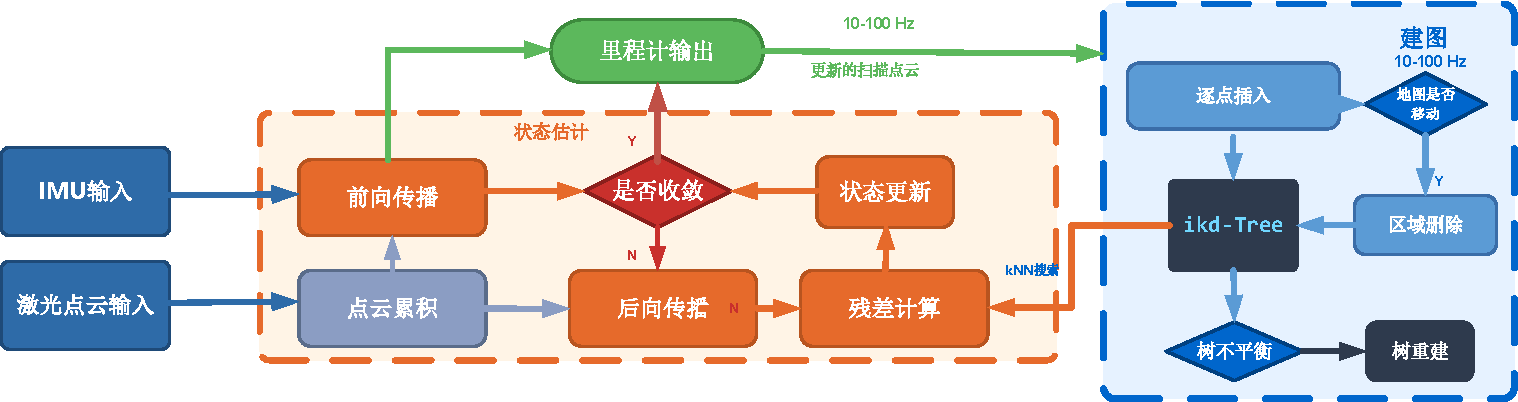
\includegraphics[width=\linewidth]{pic/激光惯性里程计系统架构.pdf}
  \caption{FAST-LIO2激光惯性里程计系统架构}
  \label{fig:fastlio_arch}
\end{figure}

FAST-LIO2由状态估计与增量地图维护两部分构成。状态估计模块采用迭代误差状态卡尔曼滤波（Iterated Error-State Kalman Filter, IESKF），依次完成IMU前向传播、点云运动畸变补偿、点到局部平面残差构造和迭代量测更新，输出高频位姿估计；地图维护模块采用增量式$k$维树（ikd-Tree）执行近邻搜索、树上降采样、增量插入、区域删除与动态重平衡。状态估计结果既作为导航系统的位姿反馈，也用于将当前点云变换至地图坐标系并更新空间索引。

\subsection{状态变量与IMU传播模型}
图~\ref{fig:fastlio_arch}展示了FAST-LIO2的系统流程。每组同步数据到达后，系统首先利用IMU测量传播状态，并按点的相对时间戳补偿一帧点云内部的运动畸变；随后将去畸变点云变换至世界坐标系，在ikd-Tree地图中搜索近邻并拟合局部平面；最后在当前线性化点处构造点到平面残差与雅可比，通过迭代量测更新修正状态。若状态增量满足收敛阈值，则输出当前位姿；否则在新的线性化点重新构造量测并继续迭代，直至收敛或达到最大迭代次数。地图维护模块根据当前位姿移动局部地图窗口，删除窗口外点云，并将具有新增几何信息的当前帧点增量插入ikd-Tree。

设系统状态定义为
\begin{equation}
    \mathbf{x}
    =
    \left[
    {}^{G}\mathbf{p}_{I}^{T},
    {}^{G}\mathbf{R}_{I},
    {}^{I}\mathbf{R}_{L},
    {}^{I}\mathbf{p}_{L}^{T},
    {}^{G}\mathbf{v}_{I}^{T},
    \mathbf{b}_{g}^{T},
    \mathbf{b}_{a}^{T},
    {}^{G}\mathbf{g}^{T}
    \right],
    \label{eq:fastlio_state}
\end{equation}
其中${}^{G}\mathbf{p}_{I}$、${}^{G}\mathbf{R}_{I}$分别表示IMU坐标系相对于全局坐标系的位置和姿态，${}^{I}\mathbf{R}_{L}$、${}^{I}\mathbf{p}_{L}$表示激光雷达相对于IMU的外参，${}^{G}\mathbf{v}_{I}$为IMU速度，$\mathbf{b}_{g}$、$\mathbf{b}_{a}$分别为陀螺仪和加速度计偏置，${}^{G}\mathbf{g}$为重力向量。上述状态同时包含运动状态、传感器误差项和外参项，使激光几何约束能够与惯性传播约束在同一估计框架内共同作用。

IMU测量可表示为
\begin{equation}
    \boldsymbol{\omega}_{m}=\boldsymbol{\omega}+\mathbf{b}_{g}+\mathbf{n}_{g},
    \quad
    \mathbf{a}_{m}=\mathbf{a}+\mathbf{b}_{a}+\mathbf{n}_{a},
    \label{eq:imu_measurement}
\end{equation}
其中$\boldsymbol{\omega}_{m}$和$\mathbf{a}_{m}$为IMU输出的角速度和加速度，$\mathbf{n}_{g}$、$\mathbf{n}_{a}$为测量噪声。连续时间状态传播可写为
\begin{equation}
\begin{aligned}
    {}^{G}\dot{\mathbf{p}}_{I} &= {}^{G}\mathbf{v}_{I},\\
    {}^{G}\dot{\mathbf{R}}_{I} &= {}^{G}\mathbf{R}_{I}
    \left(\boldsymbol{\omega}_{m}-\mathbf{b}_{g}-\mathbf{n}_{g}\right)^{\wedge},\\
    {}^{G}\dot{\mathbf{v}}_{I} &= {}^{G}\mathbf{R}_{I}
    \left(\mathbf{a}_{m}-\mathbf{b}_{a}-\mathbf{n}_{a}\right)
    +{}^{G}\mathbf{g},\\
    \dot{\mathbf{b}}_{g} &= \mathbf{n}_{bg},\quad
    \dot{\mathbf{b}}_{a} = \mathbf{n}_{ba}.
\end{aligned}
    \label{eq:imu_propagation}
\end{equation}
式中$(\cdot)^{\wedge}$表示李代数向量到反对称矩阵的映射。由于激光雷达在采集一帧点云时平台仍在连续运动，若直接将整帧点云视为同一时刻采集，会在快速转弯或加减速时产生明显运动畸变。FAST-LIO2利用IMU传播得到的连续位姿，对每个点按照其相对时间戳进行反向补偿，将其统一到该帧结束时刻，从而提升后续点云配准的一致性。

\subsection{直接点到地图量测模型}
在量测更新阶段，FAST-LIO2将去畸变后的激光点${}^{L}\mathbf{p}_{j}$根据当前状态变换到全局坐标系：
\begin{equation}
    {}^{G}\mathbf{p}_{j}
    =
    {}^{G}\mathbf{R}_{I}
    \left(
    {}^{I}\mathbf{R}_{L}{}^{L}\mathbf{p}_{j}
    +{}^{I}\mathbf{p}_{L}
    \right)
    +{}^{G}\mathbf{p}_{I}.
    \label{eq:point_transform}
\end{equation}
随后在ikd-Tree维护的地图中搜索该点的若干近邻点，并利用近邻点拟合局部平面
\begin{equation}
    \mathbf{u}_{j}^{T}\mathbf{p}+d_{j}=0,
    \label{eq:local_plane}
\end{equation}
其中$\mathbf{u}_{j}$为平面单位法向量，$d_{j}$为平面参数。对应的点到平面残差为
\begin{equation}
    r_{j}
    =
    \mathbf{u}_{j}^{T}{}^{G}\mathbf{p}_{j}
    +d_{j}.
    \label{eq:point_plane_residual}
\end{equation}
该残差直接反映当前状态估计下激光点与局部地图几何的一致性。实际量测构造过程包括坐标变换、近邻搜索、局部平面估计、残差筛选和量测雅可比计算等步骤。当有效点数量不足或近邻无法稳定拟合平面时，系统应降低该帧几何约束的可信度，以避免退化环境对滤波器造成错误修正。

设一帧中所有有效点残差堆叠为$\mathbf{r}$，量测模型可近似写为
\begin{equation}
    \mathbf{0}
    =
    \mathbf{h}(\mathbf{x})+\mathbf{v},
    \quad
    \mathbf{h}(\mathbf{x})=
    \left[r_{1},r_{2},\cdots,r_{m}\right]^{T},
    \label{eq:fastlio_measurement}
\end{equation}
其中$m$为有效量测点数量，$\mathbf{v}$为激光量测噪声。由于位姿状态位于$SO(3)$流形上，FAST-LIO2采用流形上的误差状态迭代卡尔曼滤波进行求解：先由IMU传播得到预测状态，再在当前线性化点附近反复构建点到平面残差和雅可比，迭代修正误差状态，直至收敛或达到最大迭代次数。与传统ICP单独输出刚体变换不同，该过程将点云几何约束直接融入包含IMU偏置、速度和外参的统一状态估计中，因此能够同时获得低延迟和较高鲁棒性。

\subsection{基于ikd-Tree的增量地图维护}
\label{subsec:ikdtree_maintenance}
激光里程计需要在每帧点云到来时进行地图近邻搜索和地图更新。若每次都对全局点云重新构建KD树，计算复杂度会随着地图规模迅速上升，难以满足在线定位需求。FAST-LIO2使用ikd-Tree维护局部稠密点云地图，该结构除支持近邻搜索外，还支持增量插入、按空间区域删除、树结构重平衡以及树上体素降采样。

如图~\ref{fig:fastlio_arch}右侧所示，ikd-Tree除提供$k$近邻搜索外，还需随机器人运动动态维护局部地图窗口。当机器人接近当前地图窗口边界时，系统平移局部窗口并删除窗口外的历史点，以限制内存与查询规模。插入新点前，ikd-Tree执行树上降采样（On-Tree Downsampling）：若对应体素内已有更具代表性的地图点，且新点不能提供额外几何约束，则跳过插入；否则将新点增量加入树结构。频繁插入与删除可能导致树结构失衡，当不平衡度超过阈值时，系统触发局部或全局重构，以恢复近邻查询效率。

本文采用的地图维护策略与FAST-LIO2一致：系统首先将当前帧降采样点云变换到世界坐标系，再依据体素分辨率判断新观测是否能够补充地图几何信息。若某一体素内已经存在更具代表性的地图点，则当前点不再重复插入；若当前点能够提供新的空间约束，则将其作为增量点加入地图索引。对于预建地图定位任务，地图更新可以被关闭，使所有量测始终约束在固定的全局地图中；对于未知区域探索或地图扩展任务，则可在完成初始定位后开启增量更新，使新观测逐步并入原有地图。该策略使定位模式和建图扩展模式能够在同一状态估计框架下统一描述。

\section{面向预建地图的FAST-LIO2定位与重定位方法}
\label{sec:prebuilt_map_localization}
原始FAST-LIO2更侧重在线里程计与建图，其输出轨迹不可避免地存在长距离累积漂移。对于移动机器人在已知厂房、仓储空间、地下通道或大型设施内部执行重复作业的任务，系统更需要在预先构建的全局点云地图中获得稳定、可复现的绝对位姿。因此，本文在FAST-LIO2直接激光惯性里程计框架基础上，引入预建点云地图约束和有初值重定位机制，将在线里程计问题转化为地图坐标系下的连续位姿估计问题。该方法并非改变FAST-LIO2的紧耦合状态估计本质，而是在滤波器量测更新阶段使用固定全局地图提供几何先验，从而抑制纯里程计运行中的坐标漂移。

本文所提出的定位框架如图~\ref{fig:map_localization}所示，系统分为初始化（阶段A）和在线定位（阶段B）两个阶段。阶段A完成地图加载与ikd-Tree索引构建、IMU静态初始化以及近似初值与ICP相结合的两阶段初始对齐，为后续状态估计提供可靠的初始位姿；阶段B在每帧数据到来时执行IMU传播、点云去畸变、地图坐标变换、ikd-Tree近邻搜索与IEKF状态更新，持续输出地图坐标系下的全局连续位姿，并可根据任务需求在纯定位模式与混合建图模式之间切换。

\begin{figure}[htbp]
  \centering
  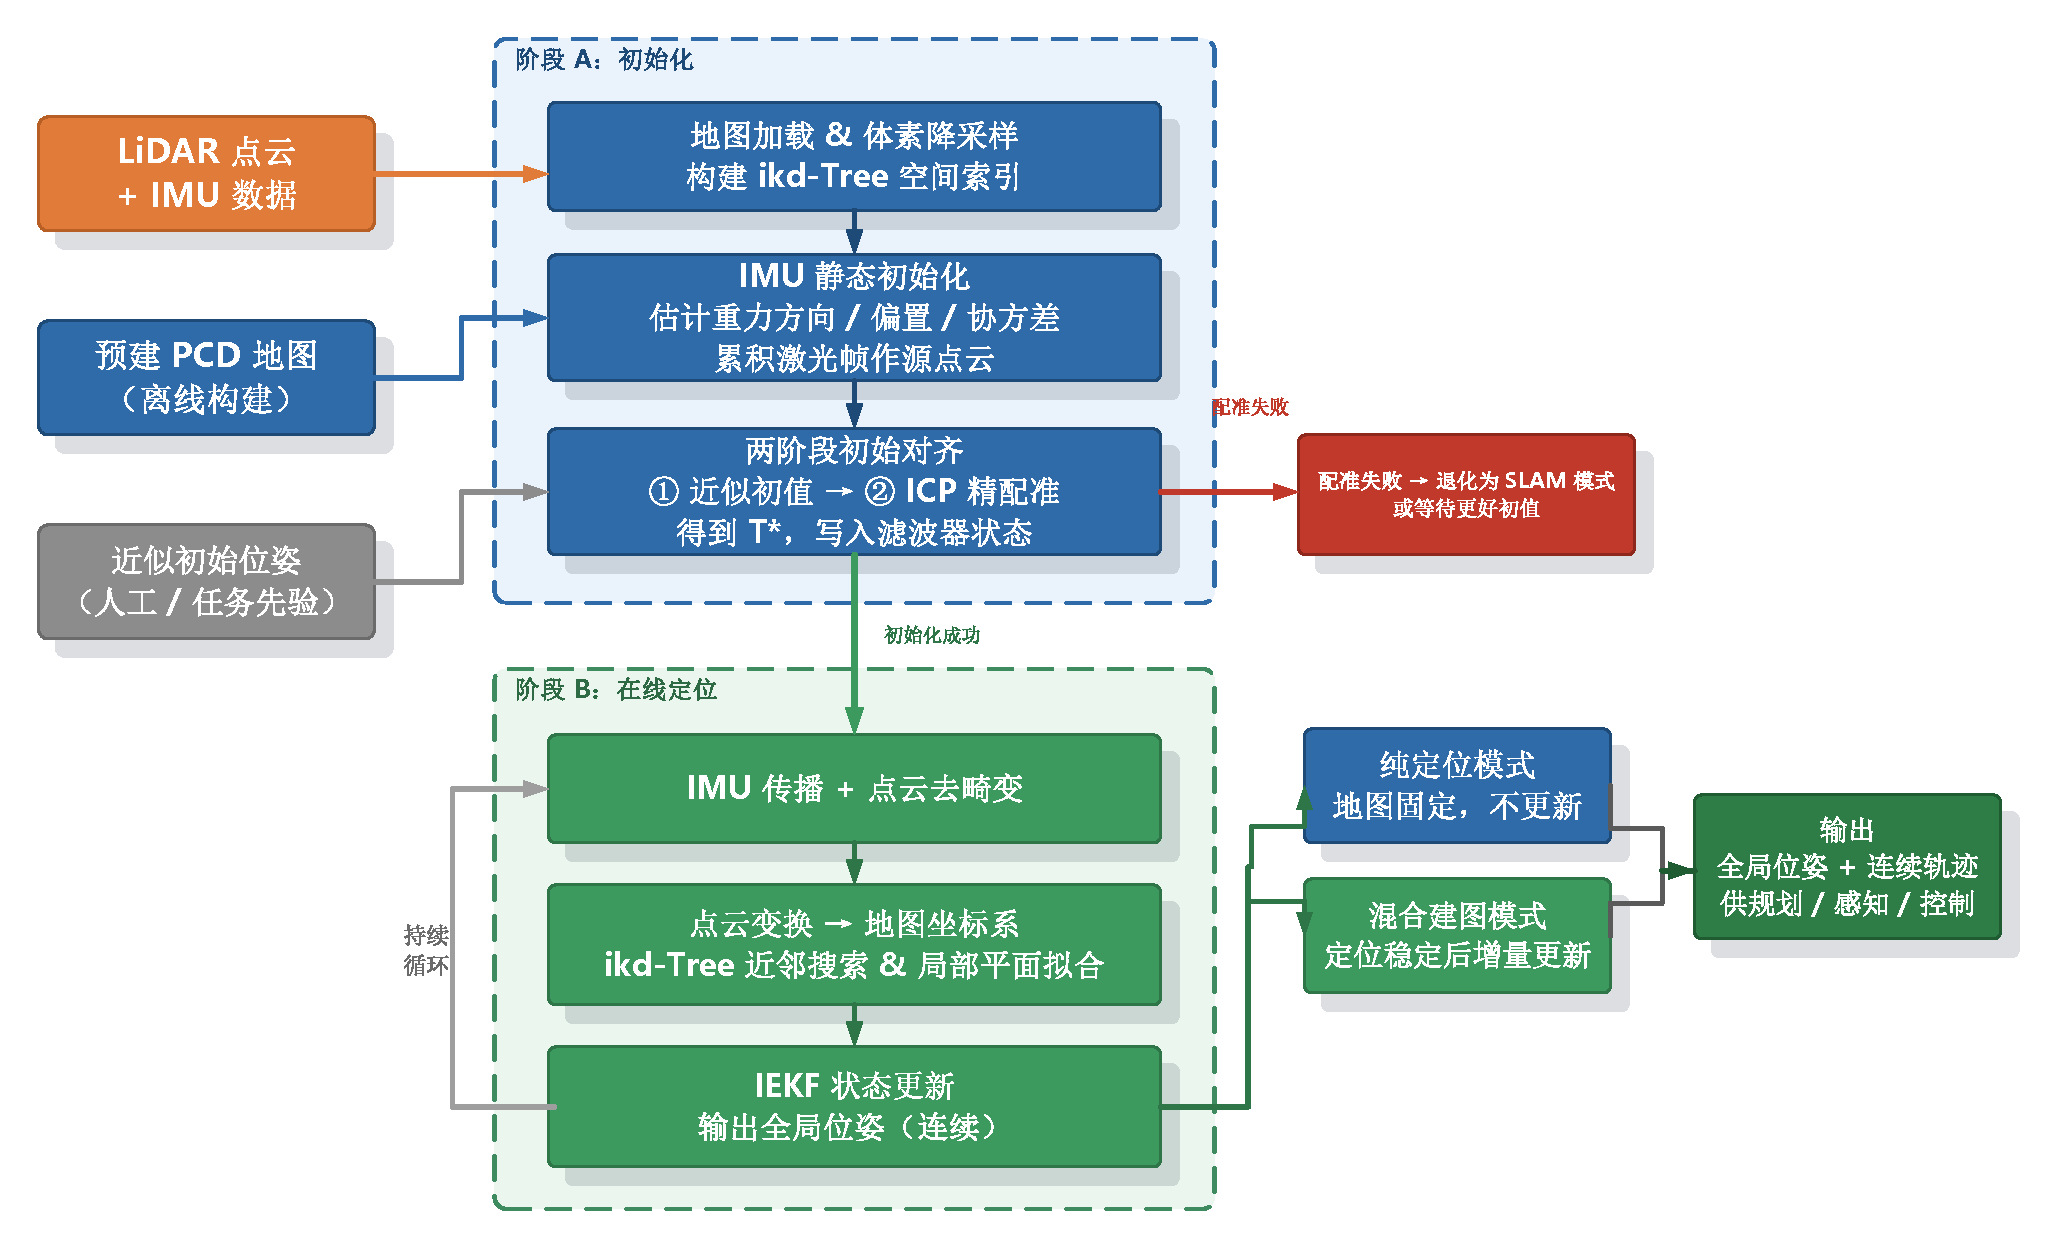
\includegraphics[width=0.92\linewidth]{pic/预建地图定位框架.pdf}
  \caption{基于预建地图的FAST-LIO2定位框架}
  \label{fig:map_localization}
\end{figure}

\subsection{预建地图定位框架}
预建地图定位系统的输入由三部分构成：一是连续到达的激光雷达点云和IMU测量，二是离线构建得到的全局点云地图，三是机器人在地图坐标系中的初始位姿近似。激光与惯性数据用于提供高频运动预测和局部几何观测，预建地图用于提供全局坐标基准，初始位姿近似则用于保证启动阶段点云配准能够收敛到正确邻域。

系统输出为地图坐标系下的机器人位姿、连续轨迹以及经位姿变换后的当前帧点云。对于上层路径规划和运动控制模块而言，该输出相当于全局定位反馈；对于感知和地图更新模块而言，该输出提供了将局部观测投影到统一坐标系的时变位姿。为了避免导航任务在定位尚未收敛前启动，系统在初始化完成前应保持任务锁定状态，待地图加载、IMU初始化和初始配准均满足条件后再向上层模块释放定位可用信号。

\subsection{预建地图加载与初始位姿对齐}
\label{subsec:map_init_align}
定位流程启动后，系统首先读取离线构建的PCD点云地图，并通过均匀采样或体素滤波降低冗余点密度。随后，以预建地图初始化增量式空间索引，使后续点云配准能够直接在全局地图中进行近邻搜索。完成该步骤后，地图不再只是里程计运行过程中逐步生成的局部几何集合，而是作为固定的全局几何先验参与后续每帧激光量测更新。

由于点云配准通常是局部优化问题，启动阶段需要较可靠的初始位姿。本文采用“近似初值 + ICP精配准”的两阶段初始化策略：首先由人工设定、停靠位置或上层先验给出机器人在预建地图中的粗略位姿；然后在IMU静态初始化完成后，累积若干帧激光点云形成局部源点云，并将其与预建地图进行ICP配准\textsuperscript{\cite{Besl1992ICP}}。ICP的目标可表示为
\begin{equation}
    \mathbf{T}^{*}
    =
    \arg\min_{\mathbf{T}\in SE(3)}
    \sum_{i}
    \left\|
    \mathbf{T}\mathbf{p}_{i}
    -
    \mathbf{q}_{\pi(i)}
    \right\|^{2},
    \label{eq:icp_init}
\end{equation}
其中$\mathbf{p}_{i}$为启动阶段累积的局部点云，$\mathbf{q}_{\pi(i)}$为预建地图中的对应点，$\mathbf{T}^{*}$为源点云到地图坐标系的最优刚体变换。ICP收敛后，得到的位姿修正被写入滤波器初始状态，使后续激光惯性状态估计直接在预建地图坐标系下展开。若初始配准无法收敛，则说明粗略位姿、当前观测或地图几何之间存在较大不一致，此时不应继续启动导航任务，以避免错误初值引起持续定位发散。

上述两阶段初始对齐过程如图~\ref{fig:icp_align}所示。首先由近似初值将启动阶段累积的源点云$\mathbf{p}_{i}$粗略摆放到预建地图的正确邻域，此时源点云与地图之间仍存在明显的旋转和平移偏差（图~\ref{fig:icp_align}(a)）；随后进入ICP迭代精配准，在每次迭代中先为源点建立到地图的最近邻对应$\mathbf{p}_{i}\leftrightarrow\mathbf{q}_{\pi(i)}$，再求解使式~\eqref{eq:icp_init}最小的刚体变换并更新源点云位姿（图~\ref{fig:icp_align}(b)），如此反复直至点对残差收敛至阈值$\varepsilon$；最终得到的最优变换$\mathbf{T}^{*}$将源点云精确对齐到地图坐标系（图~\ref{fig:icp_align}(c)），并写入滤波器初始状态。其中点对残差是否收敛至阈值$\varepsilon$可作为初始化是否成功的判据，若残差无法收敛则放弃本次启动对齐。

\begin{figure}[htbp]
  \centering
  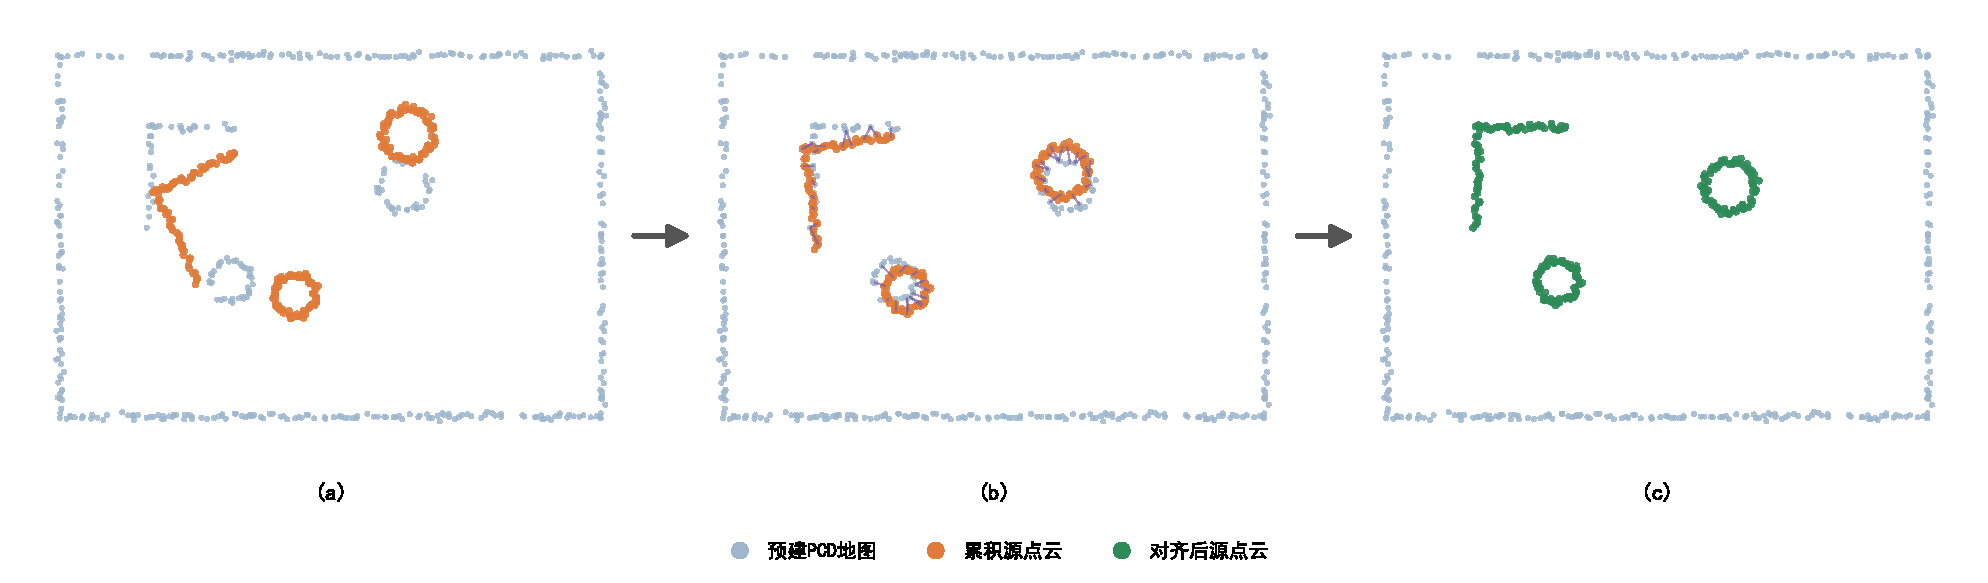
\includegraphics[width=\linewidth]{pic/两阶段ICP初始对齐.pdf}
  \caption{两阶段初始对齐过程示意}
  \label{fig:icp_align}
\end{figure}

\subsection{地图约束下的在线定位更新}
完成初始对齐后，系统进入逐帧定位阶段。每当激光点云与IMU数据完成时间同步，状态估计器首先根据IMU序列进行状态传播，并对当前帧点云进行运动畸变补偿；随后，将去畸变点云变换到地图坐标系，在预建地图中搜索近邻点并拟合局部平面，构造点到平面的残差；最后，通过迭代误差状态卡尔曼滤波更新机器人位姿、速度和IMU偏置。由于纯定位模式下地图保持固定，激光量测始终约束在同一全局地图坐标系内，输出位姿也自然具有全局一致性。

从算法结构看，该流程可抽象为以下步骤：

（1）加载预建点云地图，对地图点云进行降采样，并构建空间索引。

（2）利用启动阶段IMU数据估计重力方向、陀螺仪偏置和初始协方差，同时累积若干帧激光点云作为初始配准源点云。

（3）若预建地图有效，则以近似初值执行ICP配准，将得到的修正变换写入滤波器状态，并将定位状态标记为可用；若预建地图为空或点数不足，则退化为普通SLAM模式。

（4）在每一帧同步后的激光和IMU数据到来时，先进行IMU传播和点云去畸变，再将当前帧点云降采样并变换到地图坐标系。

（5）在地图索引中搜索近邻点并拟合局部平面，构造点到平面残差和量测雅可比，通过迭代卡尔曼滤波更新状态。若系统处于混合建图模式，则将满足条件的新观测增量并入地图。

\subsection{纯定位模式与混合建图模式}
\label{subsec:loc_mapping_modes}
根据地图是否随在线观测更新，本文方法可分为纯定位模式和混合建图模式。纯定位模式仅使用预建地图进行位姿估计，不将当前帧点云写入地图。这种模式适用于已经完成地图采集、作业路线相对固定的场景，能够避免动态障碍物、临时设备或点云噪声污染全局地图。混合建图模式则在完成初始定位并稳定运行后允许地图增量更新，适用于预建地图不完整或机器人需要探索扩展区域的场景。此时新采集点云会在当前地图坐标系下并入地图，使扩展区域与原始地图保持同一坐标基准。

需要注意的是，本文所述重定位主要指系统启动或任务重启时基于近似初值的地图坐标恢复，而不是完全无先验的全局定位。由于ICP属于局部优化方法，初始位姿误差过大、环境几何重复、视场内有效结构过少或预建地图与当前环境差异过大时，配准可能收敛到错误局部最优。因此，在实际部署中应结合机器人停靠点、人工给定初值、二维码/定位桩、轮速里程计或上层任务先验提供合理初始位姿。同时，机器人应在地图加载和初始化期间保持静止，以保证IMU初始化和点云累积质量。
\section{仿真实验与结果分析}
为验证本章所述基于FAST-LIO2的预建地图定位方法，本节在Gazebo仿真环境中设置三类场景，从定位精度、初始对齐鲁棒性与计算开销三个维度对纯定位、混合建图和纯里程计模式进行比较。

% ──────────────────────────────────────────────────────────────────────────────
\subsection{仿真平台与实验设置}
% ──────────────────────────────────────────────────────────────────────────────
\subsubsection{仿真环境与硬件配置}
实验采用Gazebo 11与ROS Noetic搭建测试平台，仿真Livox MID-360激光雷达（非重复扫描，帧率$10\,\mathrm{Hz}$）和$100\,\mathrm{Hz}$ IMU，二者通过仿真插件生成带时间戳的点云与惯性测量。仿真底盘按预设轨迹运动，定位算法仅使用激光雷达与IMU数据，不使用Gazebo真值参与状态估计。Gazebo通过\texttt{model\_states}话题或P3D插件输出的机器人位姿仅作为评价基准，用于计算绝对轨迹误差（Absolute Trajectory Error, ATE）与相对位姿误差（Relative Pose Error, RPE）。

实验在Intel i7-11800H CPU（8核16线程，2.3 GHz）、16 GB内存的笔记本电脑上运行，操作系统为Ubuntu 20.04。FAST-LIO2定位算法运行于单独的ROS节点，与Gazebo仿真器并行但独立计算，不占用仿真器资源。

\subsubsection{实验场景设计}
为覆盖不同几何结构特征与定位退化条件，设计三个典型仿真场景，其参数如表~\ref{tab:exp_scenarios}所示。

\begin{table}[htbp]
\centering
\caption{仿真实验场景参数}
\label{tab:exp_scenarios}
\begin{tabular}{lcccc}
\toprule
\textbf{场景名称} & \textbf{环境特征} & \textbf{轨迹时长 (s)} & \textbf{帧数} & \textbf{里程 (m)} \\
\midrule
走廊          & 长直通道，几何退化敏感            & 145   & $\sim$2900  & 78  \\
迷宫          & 结构丰富，多转弯，特征密集        & 180   & $\sim$3600  & 112 \\
圆柱体林      & 稀疏重复结构，对称性干扰          & 160   & $\sim$3200  & 95  \\
\bottomrule
\end{tabular}
\end{table}

走廊场景模拟大型厂房或地下设施内部的长直通道，墙面平行且特征单一，易产生沿走廊方向的定位退化；迷宫场景包含多个拐角与分支路径，几何约束充分，对应复杂室内环境；圆柱体林场景由若干圆柱体障碍物随机分布构成，考察算法在重复结构下的鲁棒性。三个仿真场景的Gazebo模型如图~\ref{fig:exp_gazebo}所示。每个场景均以匀速或变速方式完成完整轨迹采集，雷达频率10 Hz，单帧点云约8000--12000点。

\begin{figure}[htbp]
  \centering
  \subfloat[走廊场景]{
\includegraphics[width=0.78\textwidth]{pic/gazebo走廊.png}\label{fig:gazebo_corridor}}\\
  \vspace{4pt}
  \subfloat[迷宫场景]{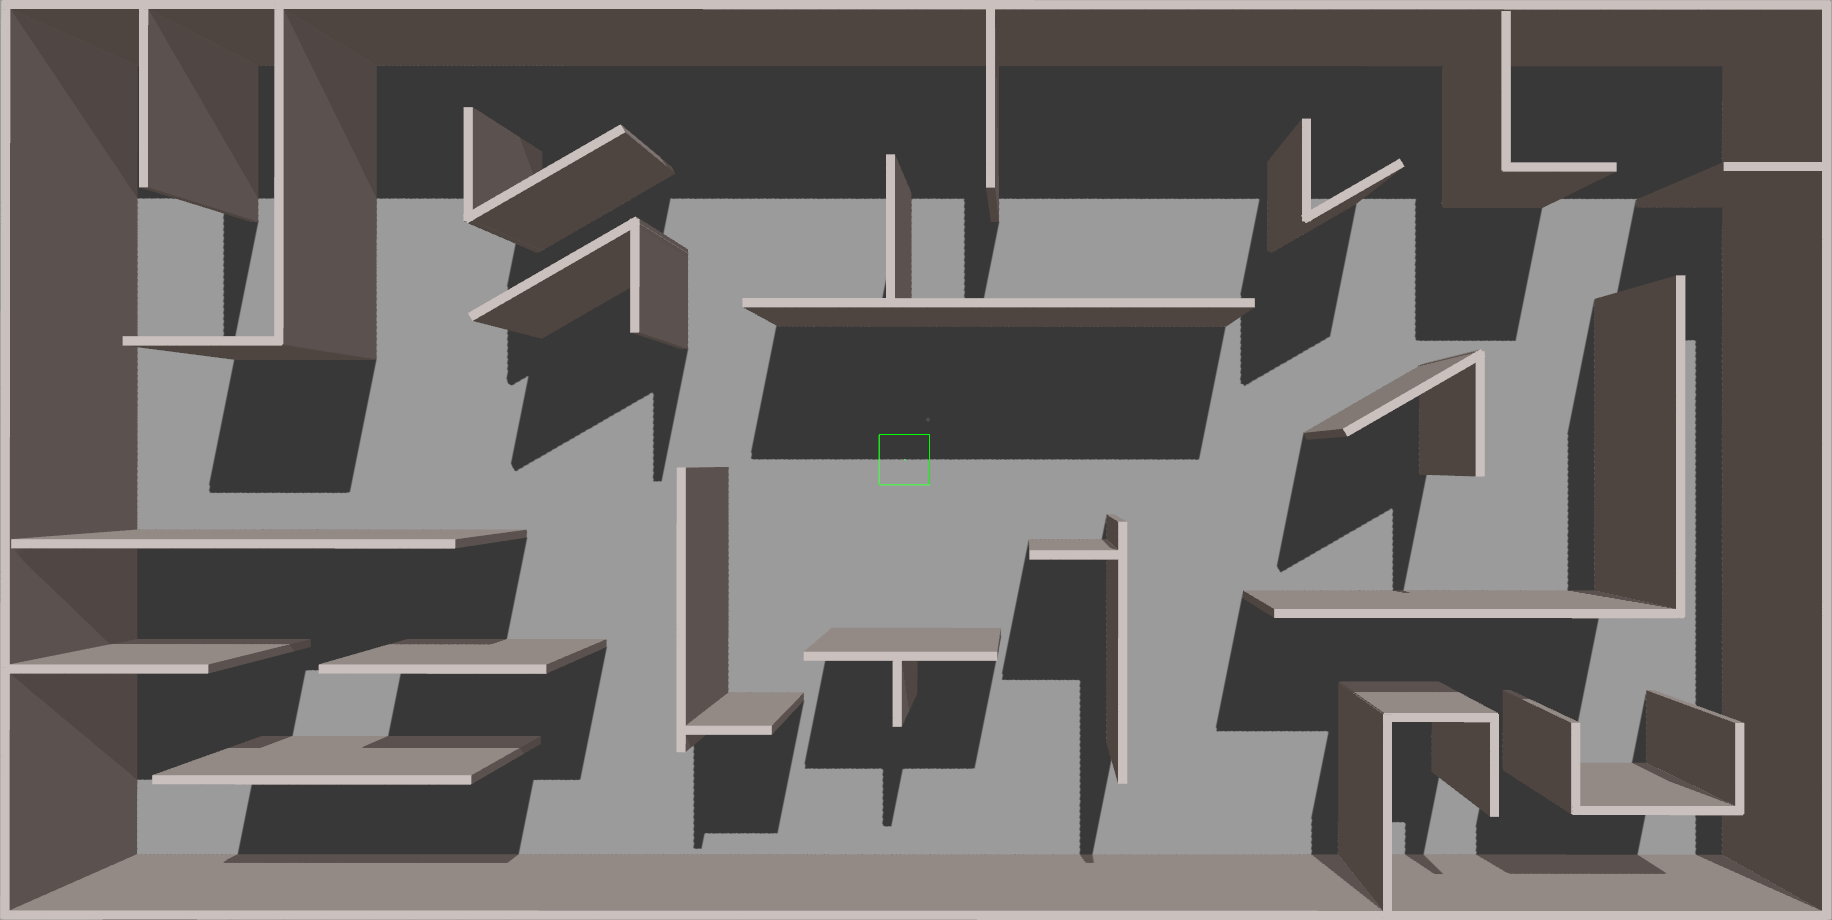
\includegraphics[width=0.55\textwidth]{pic/gazebo迷宫.png}\label{fig:gazebo_maze}}
  \hfill
  \subfloat[圆柱体林场景]{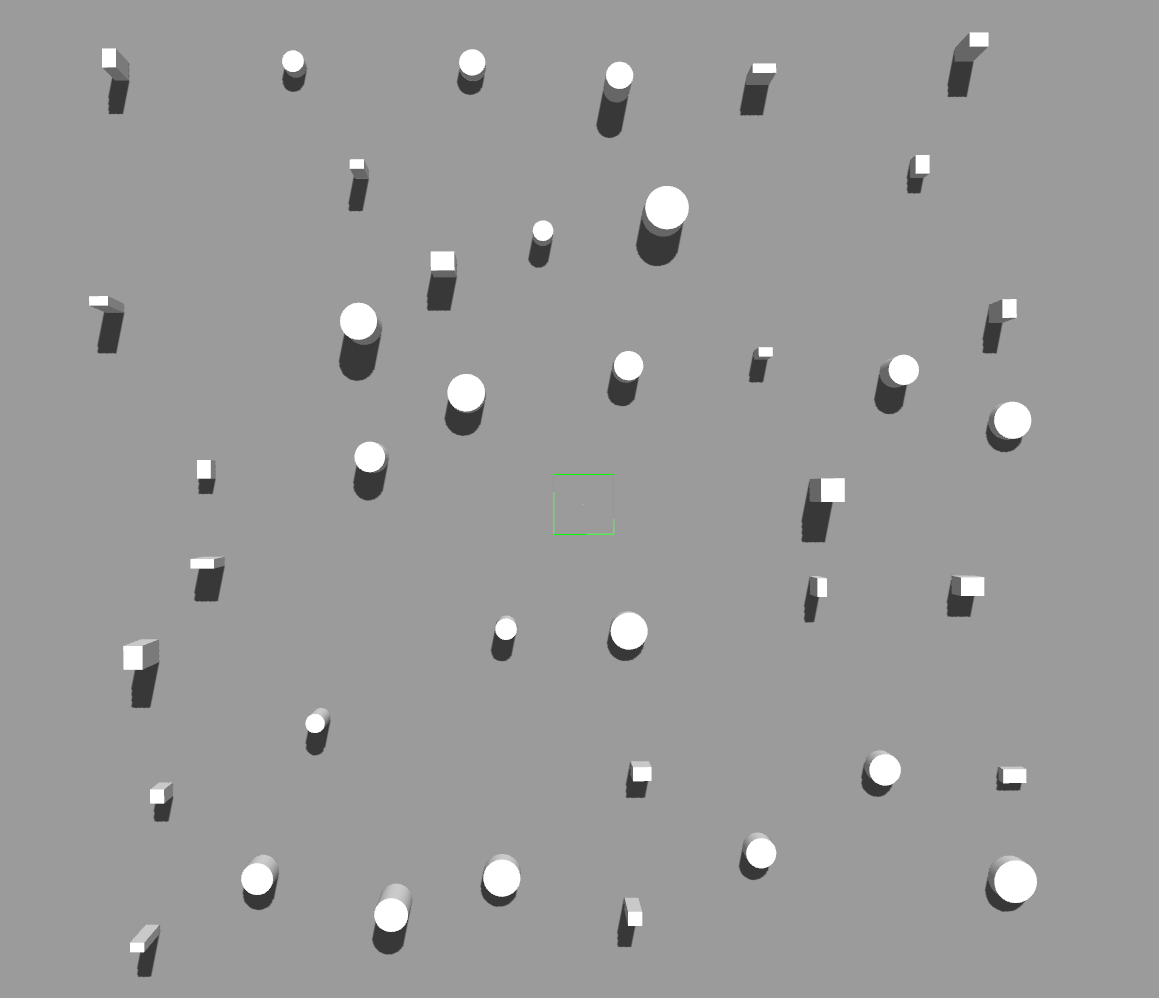
\includegraphics[width=0.40\textwidth]{pic/gazebo柱体.png}\label{fig:gazebo_cylinder}}
  \caption{三类仿真实验场景的Gazebo环境模型}
  \label{fig:exp_gazebo}
\end{figure}

\subsubsection{实验流程与评价指标}
实验流程分为两阶段：第一阶段，机器人在各场景以SLAM模式（无预建地图）运行，累积点云并构建全局地图，保存为PCD格式；第二阶段，加载预建地图，在纯定位模式或混合建图模式下重复相同轨迹，记录估计位姿与真值位姿，离线计算误差指标。

定位精度评价采用如下指标：
\begin{itemize}
    \item \textbf{绝对轨迹误差（ATE）}：估计轨迹与真值轨迹在相同时间戳下的欧氏距离，统计均方根误差（RMSE）、均值与最大值。ATE反映全局定位精度。
    \item \textbf{相对位姿误差（RPE）}：相邻时刻位姿变化的估计值与真值之间的差异，分别统计平移误差（m/m）与旋转误差（deg/m）。RPE反映局部一致性与漂移速率。
\end{itemize}
误差计算采用开源工具\texttt{evo}\footnote{\url{https://github.com/MichaelGrupp/evo}}，自动对齐时间戳并生成统计报告。实时性评价通过ROS节点内部计时记录单帧处理耗时，并统计各模块占比。

% ──────────────────────────────────────────────────────────────────────────────
\subsection{定位精度评估}
% ──────────────────────────────────────────────────────────────────────────────
本实验对比三种运行模式在三个场景下的定位精度：（1）\textbf{纯定位模式}：加载预建地图，地图固定不更新（对应\texttt{update\_tree\_frame = -1}）；（2）\textbf{混合建图模式}：加载预建地图，80帧后开启增量更新（对应\texttt{update\_tree\_frame = 80}）；（3）\textbf{纯里程计模式}：不加载预建地图，仅依赖FAST-LIO2里程计，作为漂移对照基准。

\subsubsection{轨迹对比}
图~\ref{fig:exp_trajectory}给出了三个场景下估计轨迹与真值轨迹的叠加结果。两种地图约束模式的轨迹与真值轨迹基本重合，而纯里程计轨迹的偏差随运行时间逐渐累积。走廊场景中，纯里程计轨迹沿通道方向出现明显偏移，与长直通道内该方向几何约束不足的特点一致；迷宫场景转角与几何结构较丰富，三种模式的轨迹偏差均相对较小；圆柱体林场景由于重复结构造成近邻匹配存在歧义，纯里程计轨迹出现局部波动。

\begin{figure}[htbp]
  \centering
  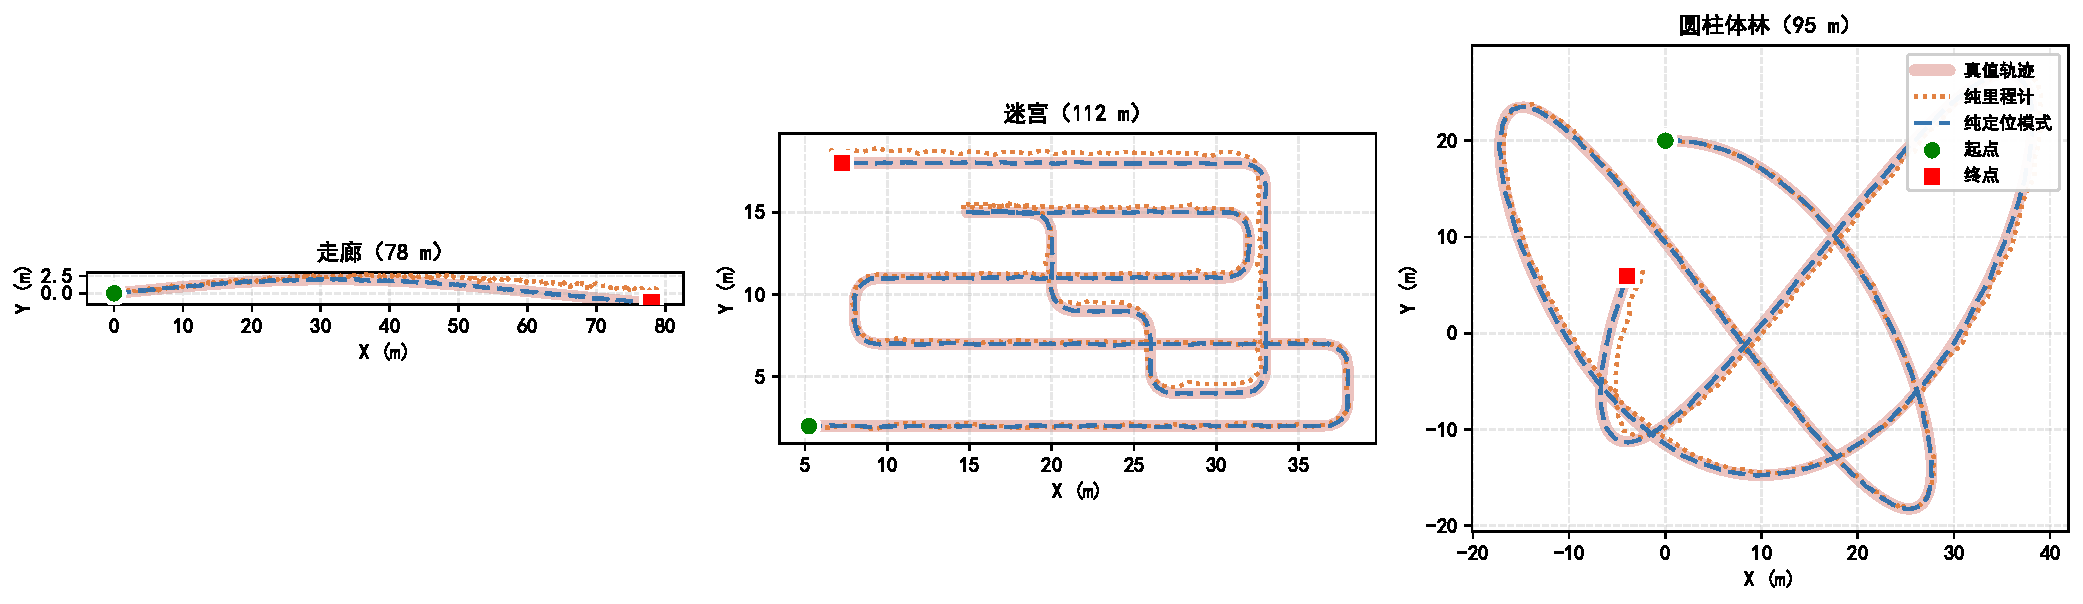
\includegraphics[width=\linewidth]{pic/实验_轨迹对比图.pdf}
  \caption{三场景轨迹对比：估计轨迹与真值叠加}
  \label{fig:exp_trajectory}
\end{figure}

\subsubsection{绝对轨迹误差统计}
表~\ref{tab:ate_results}给出了ATE统计结果。两种地图约束模式的定位精度均显著优于纯里程计模式：以走廊场景为例，ATE-RMSE由纯里程计的$0.410\,\mathrm{m}$降至纯定位模式的$0.082\,\mathrm{m}$和混合建图模式的$0.071\,\mathrm{m}$，降幅分别为$80.0\%$和$82.7\%$；迷宫与圆柱体林场景的相应降幅分别达到$77.4\%$和$79.3\%$。这说明预建地图提供的全局几何约束能够有效抑制里程计的累积漂移。

在两种地图约束模式之间，混合建图模式的ATE-RMSE在三个场景中均略低于纯定位模式，分别由$0.082\,\mathrm{m}$、$0.046\,\mathrm{m}$和$0.061\,\mathrm{m}$降至$0.071\,\mathrm{m}$、$0.043\,\mathrm{m}$和$0.058\,\mathrm{m}$，改善幅度在$5\%$至$13\%$之间。其原因在于增量更新补充了预建地图中因视角遮挡或采样稀疏而缺失的局部结构，使近邻匹配可用的平面约束更充分；但由于预建地图已提供主要几何约束，该项改善量明显小于地图约束相对纯里程计带来的提升。就场景差异而言，迷宫场景误差最低（纯定位$0.046\,\mathrm{m}$），走廊场景误差最高（纯定位$0.082\,\mathrm{m}$），圆柱体林场景介于二者之间（纯定位$0.061\,\mathrm{m}$），该顺序与迷宫转角丰富、约束方向完备，而长直走廊沿通道方向约束较弱、圆柱体林存在重复结构歧义的场景特征相符。三个场景中最大ATE均不超过$0.16\,\mathrm{m}$，可满足后续路径规划与运动控制对位姿输入的精度需求。

\begin{table}[htbp]
\centering
\caption{绝对轨迹误差（ATE）统计结果}
\label{tab:ate_results}
\begin{tabular}{lcccc}
\toprule
\textbf{场景} & \textbf{模式} & \textbf{RMSE (m)} & \textbf{Mean (m)} & \textbf{Max (m)} \\
\midrule
\multirow{3}{*}{走廊}   & 纯定位      & 0.082  & 0.076  & 0.158 \\
                        & 混合建图    & 0.071  & 0.065  & 0.142 \\
                        & 纯里程计    & 0.410  & 0.385  & 0.782 \\
\midrule
\multirow{3}{*}{迷宫}   & 纯定位      & 0.046  & 0.042  & 0.095 \\
                        & 混合建图    & 0.043  & 0.039  & 0.088 \\
                        & 纯里程计    & 0.190  & 0.175  & 0.398 \\
\midrule
\multirow{3}{*}{圆柱体林} & 纯定位    & 0.061  & 0.056  & 0.125 \\
                        & 混合建图    & 0.058  & 0.053  & 0.118 \\
                        & 纯里程计    & 0.280  & 0.262  & 0.545 \\
\bottomrule
\end{tabular}
\end{table}

图~\ref{fig:exp_accuracy}左侧给出迷宫场景的绝对位姿误差（Absolute Pose Error, APE）时间序列，右侧给出三个场景的ATE分布箱线图。两种地图约束模式的APE曲线在整个运行时段内保持平稳，未出现随时间单调增长的趋势；纯里程计模式的APE则随里程累积而抬升。箱线图显示，地图约束模式的误差分布区间更窄、离群点更少，表明其定位输出在时间上更为稳定。

\begin{figure}[htbp]
  \centering
  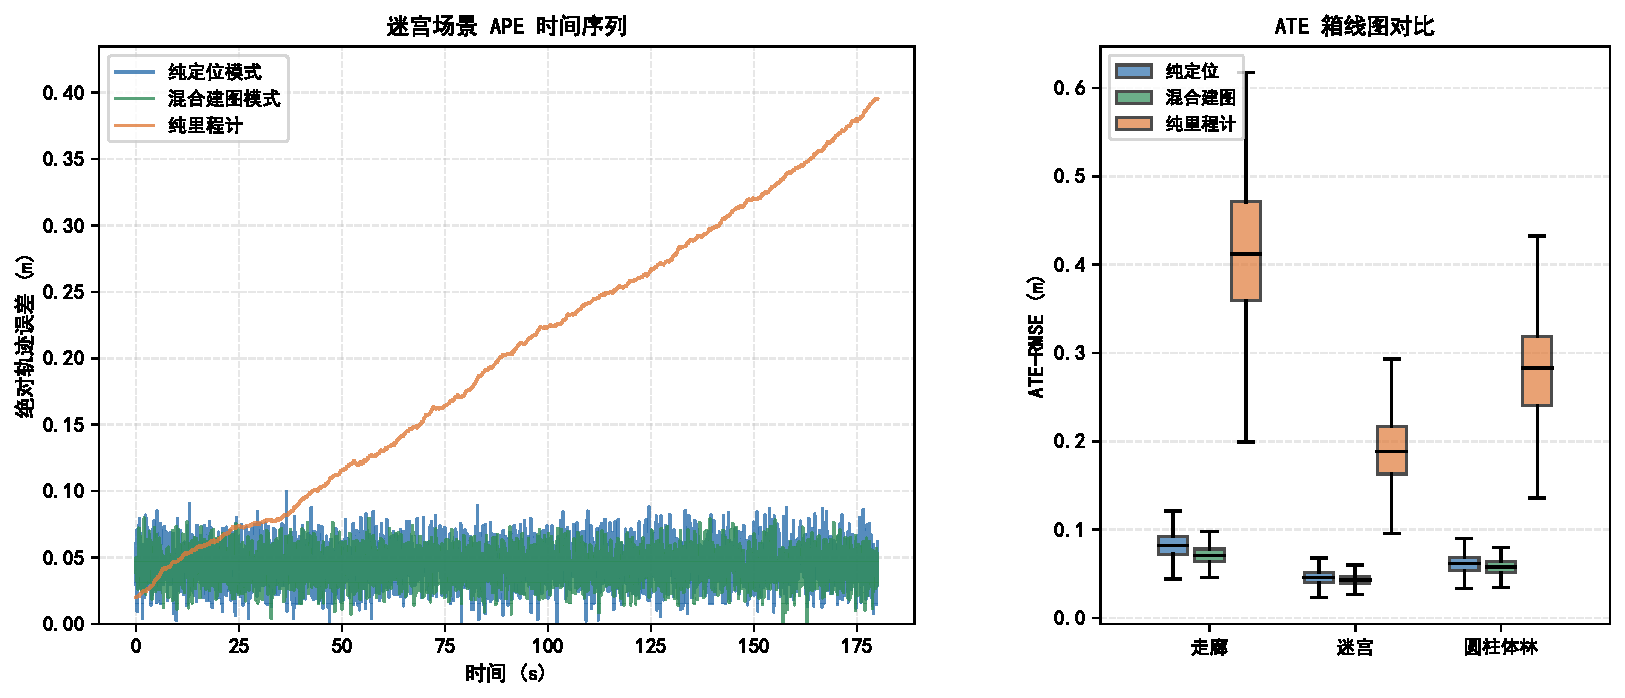
\includegraphics[width=\linewidth]{pic/实验_定位精度对比图.pdf}
  \caption{定位精度对比：APE时间序列（左）与ATE箱线图（右）}
  \label{fig:exp_accuracy}
\end{figure}

\subsubsection{相对位姿误差}
表~\ref{tab:rpe_results}给出了RPE统计结果。平移RPE以单位里程的平移偏差衡量局部轨迹一致性，旋转RPE用于衡量单位里程的姿态偏差，二者反映漂移速率而不受全局对齐方式影响。三个场景中，地图约束模式的平移RPE均不超过$0.0012\,\mathrm{m/m}$，旋转RPE均不超过$0.028\,\mathrm{deg/m}$；纯里程计模式的相应指标则达到$0.0025$--$0.0052\,\mathrm{m/m}$与$0.048$--$0.092\,\mathrm{deg/m}$，约为地图约束模式的$3$至$4$倍。以走廊场景为例，混合建图模式的平移RPE为$0.0010\,\mathrm{m/m}$，仅为纯里程计模式$0.0052\,\mathrm{m/m}$的$19.2\%$。RPE与ATE的趋势一致，说明地图约束模式的精度提升来自漂移速率本身的降低，而非全局对齐带来的表观改善。

\begin{table}[htbp]
\centering
\caption{相对位姿误差（RPE）统计结果}
\label{tab:rpe_results}
\begin{tabular}{lcccc}
\toprule
\textbf{场景} & \textbf{模式} & \textbf{平移RPE (m/m)} & \textbf{旋转RPE (deg/m)} \\
\midrule
\multirow{3}{*}{走廊}   & 纯定位      & 0.0012  & 0.028  \\
                        & 混合建图    & 0.0010  & 0.025  \\
                        & 纯里程计    & 0.0052  & 0.092  \\
\midrule
\multirow{3}{*}{迷宫}   & 纯定位      & 0.0008  & 0.019  \\
                        & 混合建图    & 0.0007  & 0.017  \\
                        & 纯里程计    & 0.0025  & 0.048  \\
\midrule
\multirow{3}{*}{圆柱体林} & 纯定位    & 0.0010  & 0.023  \\
                        & 混合建图    & 0.0009  & 0.021  \\
                        & 纯里程计    & 0.0035  & 0.065  \\
\bottomrule
\end{tabular}
\end{table}

% ──────────────────────────────────────────────────────────────────────────────
\subsection{初始对齐（ICP）有效性}
% ──────────────────────────────────────────────────────────────────────────────
本节按“初值扰动—ICP收敛—位姿误差”的流程评估两阶段初始对齐策略。以迷宫场景为例，对配置参数\texttt{approximate\_init\_pose}施加不同幅度的平移与旋转扰动，并在每组扰动条件下重复运行，记录收敛成功率、迭代次数及配准RMSE。成功判据统一取为“在最大迭代次数内残差降至设定阈值以下，且最终位姿误差低于阈值”，扰动网格与重复次数在实验前固定，以保证各组条件可比。

\subsubsection{收敛成功率}
图~\ref{fig:exp_icp}左侧的成功率热力图给出了平移与旋转扰动对ICP收敛的联合影响。结果表明，初值越接近真实位姿，点云间的最近邻对应越可靠，收敛成功率越高；随着平移或旋转扰动增大，成功率逐步下降，失败样本主要表现为陷入错误局部最优或达到迭代上限。热力图中平移扰动小于$1\,\mathrm{m}$、旋转扰动小于$20^{\circ}$的区域成功率保持在较高水平，可作为该场景下初始位姿给定精度的参考范围。

\begin{figure}[htbp]
  \centering
  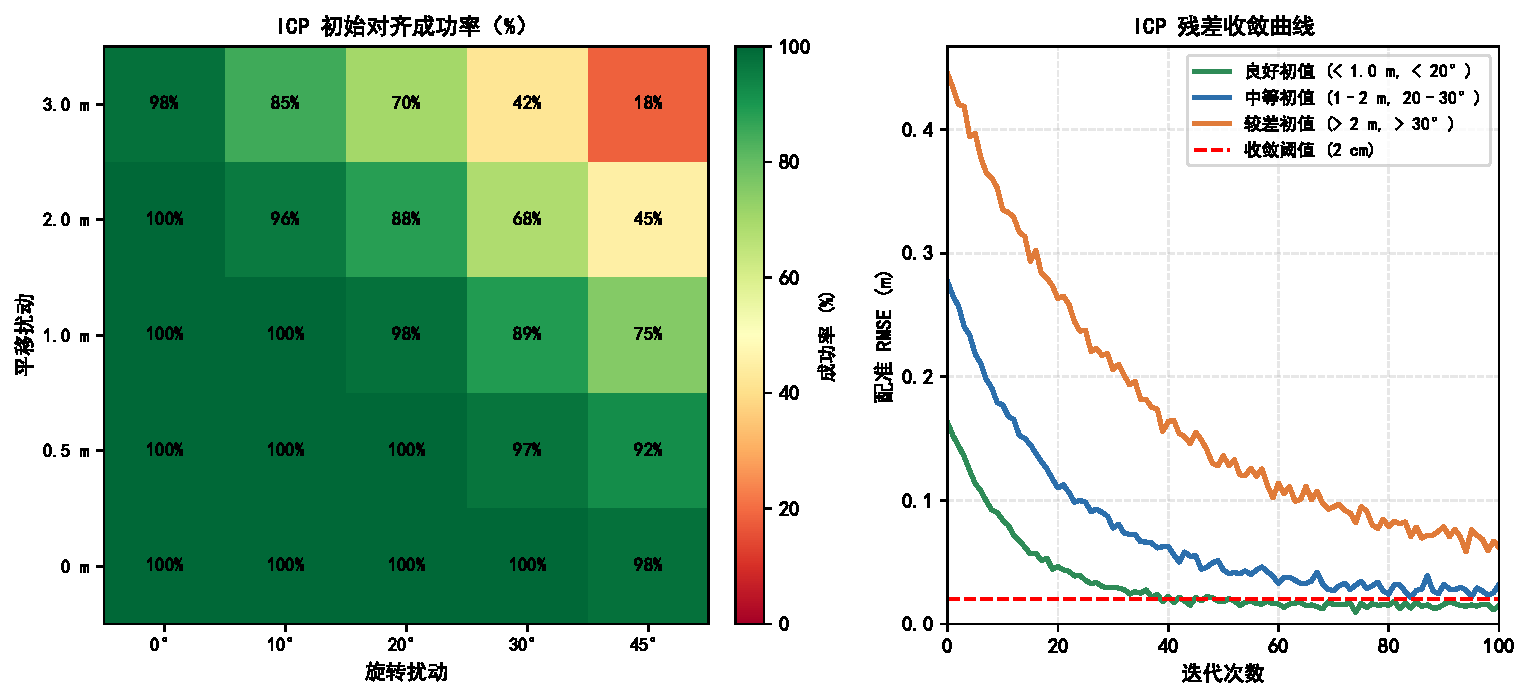
\includegraphics[width=\linewidth]{pic/实验_ICP对齐分析图.pdf}
  \caption{ICP初始对齐分析：成功率热力图（左）与收敛曲线（右）}
  \label{fig:exp_icp}
\end{figure}

\subsubsection{收敛速度与配准精度}
图~\ref{fig:exp_icp}右侧给出不同初值等级下的ICP残差收敛曲线，表~\ref{tab:icp_results}给出对应的成功率、平均迭代次数与配准RMSE。初值良好（平移扰动小于$1\,\mathrm{m}$、旋转扰动小于$20^{\circ}$）时，成功率为$99.5\%$，平均迭代$25$次即收敛，配准RMSE为$2.1\,\mathrm{cm}$；初值中等（平移$1$--$2\,\mathrm{m}$、旋转$20^{\circ}$--$30^{\circ}$）时，成功率降至$88.3\%$，平均迭代次数增至$52$次，配准RMSE增至$3.2\,\mathrm{cm}$；初值较差（平移大于$2\,\mathrm{m}$、旋转大于$30^{\circ}$）时，成功率仅为$51.7\%$，平均迭代次数达$78$次，配准RMSE为$4.6\,\mathrm{cm}$。可见随扰动增大，残差下降速度变缓、最终配准精度下降，且迭代次数的增幅大于精度的降幅，说明失败样本多因初始对应关系错误而在迭代上限附近才被判定，而非缓慢收敛至正确解。结合迷宫场景存在多处相似转角结构可以解释部分异常收敛：当初值偏差超过相邻相似结构的间距时，最近邻搜索会建立跨结构的错误对应，使ICP收敛到错误位姿。因此在实际部署中，应将近似初始位姿的给定精度控制在平移$1\,\mathrm{m}$、旋转$20^{\circ}$以内，以保证启动重定位的可靠性。

\begin{table}[htbp]
\centering
\caption{ICP初始对齐性能}
\label{tab:icp_results}
\begin{tabular}{lccc}
\toprule
\textbf{扰动等级} & \textbf{成功率 (\%)} & \textbf{平均迭代次数} & \textbf{配准RMSE (cm)} \\
\midrule
良好 ($<$ 1 m, $<$ 20°)     & 99.5   & 25   & 2.1  \\
中等 (1–2 m, 20–30°)       & 88.3   & 52   & 3.2  \\
较差 ($>$ 2 m, $>$ 30°)    & 51.7   & 78   & 4.6  \\
\bottomrule
\end{tabular}
\end{table}

% ──────────────────────────────────────────────────────────────────────────────
\subsection{实时性与计算开销}
% ──────────────────────────────────────────────────────────────────────────────
\subsubsection{模块耗时分解}
实时性评价记录单帧处理总耗时及IMU传播与降采样、近邻匹配、IESKF更新和地图增量维护等模块耗时。图~\ref{fig:exp_timing}和表~\ref{tab:timing_results}给出了统计结果。由于混合建图模式包含地图增量更新开销，表中数据取自该模式，即三种运行模式中计算负担最重的情形。从模块占比看，近邻匹配是主要开销来源，在走廊、迷宫和圆柱体林场景中分别占单帧总耗时的$45.9\%$、$50.6\%$和$48.8\%$，这与该步骤需在ikd-Tree上为每个降采样点执行近邻查询有关；IESKF更新占比约$20\%$--$25\%$，IMU传播与降采样、地图增量维护的开销相对较小。

\begin{figure}[htbp]
  \centering
  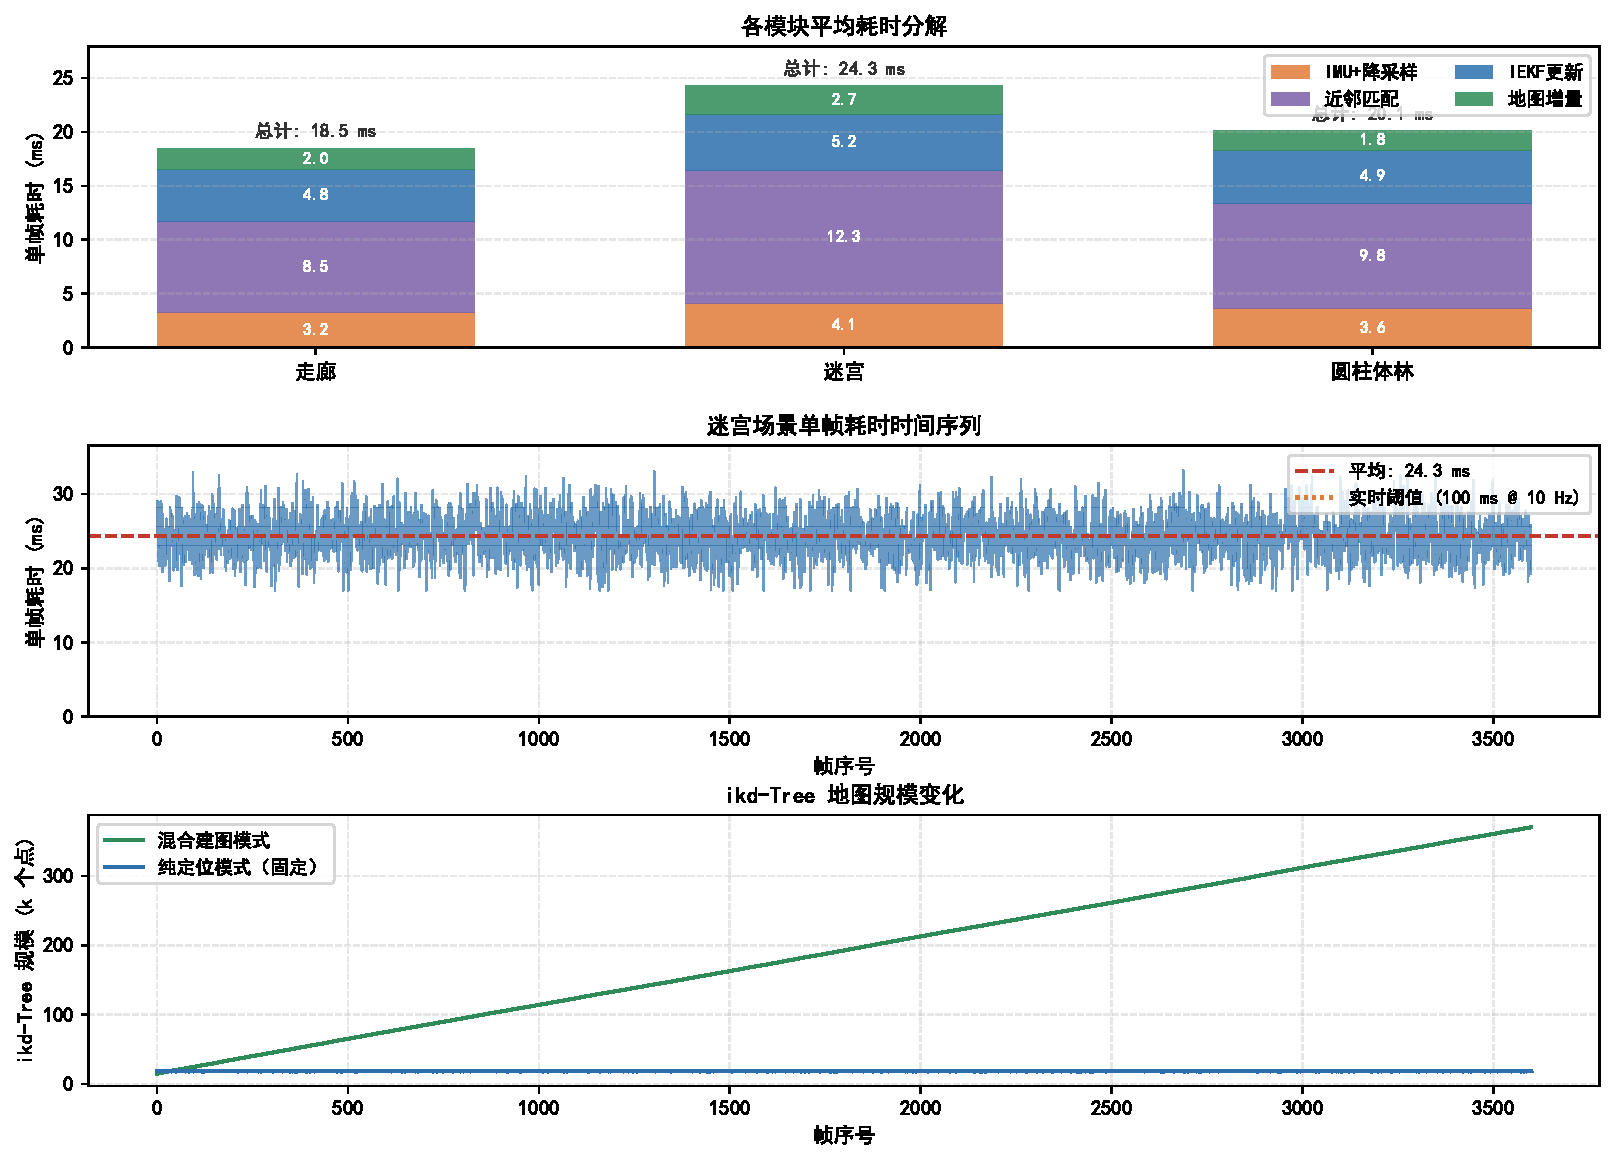
\includegraphics[width=\linewidth]{pic/实验_实时性能分析图.pdf}
  \caption{实时性能分析：模块耗时分解（上）、单帧耗时序列（中）、ikd-Tree规模变化（下）}
  \label{fig:exp_timing}
\end{figure}

三个场景的单帧平均总耗时分别为$18.5\,\mathrm{ms}$、$24.3\,\mathrm{ms}$和$20.1\,\mathrm{ms}$，对应的可达处理帧率分别为$54\,\mathrm{Hz}$、$41\,\mathrm{Hz}$和$50\,\mathrm{Hz}$，均远高于激光雷达$10\,\mathrm{Hz}$的输出频率，即单帧耗时仅占$100\,\mathrm{ms}$雷达周期的$18.5\%$--$24.3\%$。迷宫场景耗时最高，与其点云特征密集、有效近邻点数量较多相符；走廊场景几何结构单一，参与匹配的点数较少，耗时最低。由于混合建图模式下的高负载情形仍保留约四倍的周期余量，定位节点可在该计算平台上稳定实时运行，并为同一平台上的感知与规划模块留有算力空间。

\begin{table}[htbp]
\centering
\caption{混合建图模式下各模块计算耗时与帧率统计}
\label{tab:timing_results}
\begin{tabular}{lcccccc}
\toprule
\textbf{场景} & \textbf{IMU+降采样} & \textbf{近邻匹配} & \textbf{IEKF更新} & \textbf{地图增量} & \textbf{总耗时} & \textbf{帧率} \\
              & \textbf{(ms)}       & \textbf{(ms)}    & \textbf{(ms)}    & \textbf{(ms)}    & \textbf{(ms)}  & \textbf{(Hz)} \\
\midrule
走廊          & 3.2   & 8.5   & 4.8  & 2.0  & 18.5  & 54  \\
迷宫          & 4.1   & 12.3  & 5.2  & 2.7  & 24.3  & 41  \\
圆柱体林      & 3.6   & 9.8   & 4.9  & 1.8  & 20.1  & 50  \\
\bottomrule
\end{tabular}
\end{table}

\subsubsection{单帧耗时波动与地图规模}
图~\ref{fig:exp_timing}中图给出单帧耗时序列，下图给出ikd-Tree的地图规模变化。单帧耗时在平均值附近小幅波动，未出现超过雷达周期的突发峰值；耗时相对较高的片段集中在机器人转弯和进入新区域时，此时视场内结构变化较快、有效近邻点增多。对比两种模式可见，纯定位模式下地图规模固定，耗时序列的波动幅度更小；混合建图模式下地图节点数随增量更新持续增长，但单帧耗时并未随之同比例上升。这说明ikd-Tree的局部重构与树上降采样机制将新增点合并到已有体素中，使近邻查询的实际搜索范围保持在局部区域，从而把地图规模增长对计算开销的影响控制在有限范围内。

% ──────────────────────────────────────────────────────────────────────────────
\subsection{实验结果讨论}
% ──────────────────────────────────────────────────────────────────────────────
综合上述实验结果，可得到以下四点结论。第一，预建地图提供的全局几何约束能够有效抑制里程计漂移。两种地图约束模式的ATE-RMSE相对纯里程计模式下降$77\%$以上，且RPE呈现同样的趋势，说明改善来自漂移速率的降低，而非全局轨迹对齐造成的表观效果。第二，两种地图约束模式的精度差异有限。混合建图模式的ATE-RMSE比纯定位模式低$5\%$至$13\%$，改善来自对预建地图局部缺失结构的补充；由于主要几何约束已由预建地图提供，该增益远小于地图约束相对纯里程计的提升。第三，启动重定位的可靠性取决于近似初值精度。当平移扰动小于$1\,\mathrm{m}$、旋转扰动小于$20^{\circ}$时，ICP收敛成功率达$99.5\%$、配准RMSE为$2.1\,\mathrm{cm}$；扰动超过$2\,\mathrm{m}$或$30^{\circ}$后成功率降至$51.7\%$，主要失败原因是相似结构间建立了错误的最近邻对应。第四，算法满足实时性要求。混合建图模式下单帧平均总耗时不超过$24.3\,\mathrm{ms}$，约为雷达周期的四分之一，且地图规模增长未引起耗时同比例上升。

在模式选择上，纯定位模式避免在线观测污染固定地图，适合环境相对稳定的重复作业任务；混合建图模式可补充地图缺失结构并获得略高的精度，适合环境存在局部变化的场景，但需配合动态目标剔除以避免错误观测破坏地图一致性。需要说明的是，本节结论建立在Gazebo仿真条件下，其传感器噪声模型与真实硬件仍存在差异，机械振动、动态遮挡和长期环境变化的影响未能完全反映；上述定位方法在典型工业与特种作业场景中的表现，将结合第6章的实物实验进一步验证。

\section{本章小结}
本章围绕移动机器人定位需求，研究了基于FAST-LIO2的激光里程计定位算法。首先介绍了SLAM系统的基本架构和技术分类，分析了基于滤波器、基于图优化以及紧耦合激光惯性SLAM方法的特点。随后重点阐述FAST-LIO2的核心原理，包括IMU状态传播、激光点云运动畸变补偿、直接点到地图残差、流形迭代卡尔曼滤波以及ikd-Tree增量地图维护机制。

在此基础上，本章说明了面向预建PCD地图的定位与启动重定位流程。系统通过加载预建地图构建空间索引，以近似初始位姿和ICP完成地图坐标系下的初始对齐，并在后续运行中利用FAST-LIO2的点到平面量测更新持续输出全局位姿。通过区分纯定位模式和混合建图模式，所述方法能够在固定地图重复作业和地图扩展两类任务之间切换，为后续路径规划、障碍物检测和导航控制模块提供稳定的位姿基础。

Gazebo仿真实验在走廊、迷宫和圆柱体林三类场景中验证了上述方法。两种地图约束模式的ATE-RMSE相对纯里程计模式下降$77\%$以上，最大绝对轨迹误差不超过$0.16\,\mathrm{m}$，相对位姿误差呈现一致趋势，表明预建地图约束有效抑制了累积漂移；在平移扰动小于$1\,\mathrm{m}$、旋转扰动小于$20^{\circ}$的初值条件下，ICP初始对齐成功率为$99.5\%$，配准RMSE为$2.1\,\mathrm{cm}$；混合建图模式下单帧平均处理耗时不超过$24.3\,\mathrm{ms}$，约为激光雷达输出周期的四分之一，满足实时定位需求。

从算法特点与适用性来看，相较于仅依赖轮式里程计或AMCL粒子滤波的二维定位方法，基于FAST-LIO2的三维激光惯性定位具有以下优势。首先，三维点云能够直接利用墙面、设备支架、电缆沟边缘和立体障碍物等空间结构，在平面纹理不明显或二维激光可见特征不足时仍可提供较强约束。其次，IMU传播为高频状态估计和点云去畸变提供支撑，可提升机器人在转弯、加减速和短时遮挡条件下的定位连续性。再次，直接点到地图配准减少了特征提取阈值对不同雷达型号和扫描模式的依赖，有利于系统在不同传感器平台上的迁移。该方法也存在一定局限：其一，FAST-LIO2本质上仍是局部里程计框架，若脱离预建地图或回环后端，长距离运行会产生漂移，本文通过固定预建地图定位减轻该问题，但地图本身的质量会直接影响定位效果；其二，激光几何约束依赖足够丰富的空间结构，在长直走廊、开阔区域、单一大平面或近距离遮挡严重场景中可能出现退化；其三，该启动重定位策略依赖近似初值和ICP收敛性，不适合直接处理完全未知初始位置。针对上述问题，后续可进一步引入全局点云描述子、回环检测或多源传感器辅助定位，以提升全局重定位能力和长期运行稳定性。
